\documentclass[tikz,border=5mm]{standalone}
\usepackage{pgfplots}
\pgfplotsset{compat=1.18}
\usepackage{amsmath}
\usetikzlibrary{arrows.meta}

\begin{document}
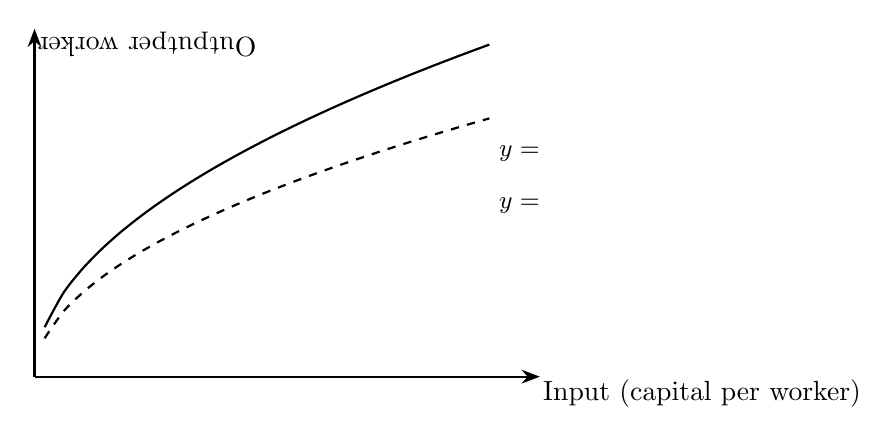
\begin{tikzpicture}
    \begin{axis}[
        width=8cm, height=6cm,
        axis lines=left,
        axis line style={-Stealth, thick},
        xmin=0, xmax=5,
        ymin=0, ymax=4,
        xtick=\empty, ytick=\empty,
        xlabel style={at={(1,0)}, anchor=north west, inner sep=1pt},
        ylabel style={at={(0,1)}, anchor=south east, rotate=90, inner sep=1pt},
        xlabel={Input (capital per worker)},
        ylabel={Output\\per worker},
        every axis plot/.append style={thick}
    ]
    
    % 上方曲线
    \addplot[black, thick, smooth, domain=0.1:4.5] {1.8*sqrt(x)};
    \node[right, font=\small] at (axis cs:4.5,2.6) {$y = G(N^u)f(k)$};
    
    % 下方曲线
    \addplot[black, thick, dashed, smooth, domain=0.1:4.5] {1.4*sqrt(x)};
    \node[right, font=\small] at (axis cs:4.5,2.0) {$y = G(N)f(k)$};
    
    % 坐标轴变量标记
    \node[below] at (axis cs:4.8,-0.1) {$k$};
    \node[left] at (axis cs:-0.1,3.8) {$y$};
    
    \end{axis}
\end{tikzpicture}
\end{document}